\chapter{Stecker und Anschlusspläne}
Der siebenpolige KF2510-Stecker ist auf der Platine nummeriert. Die Ansicht auf dem Foto und die Pinnummern verwenden, nicht allein die Kabelfarben. Pin 1: K30/KL30, Versorgung; Pin 2: V2; Pin 3: V1; Pin 4: 1WRE, One-Wire; Pin 5: KL, reservierte K-Line; Pin 6: +5 V Ausgang, maximal 30 mA; Pin 7: GND, Masse.

Der Voltmeter-Anschlussplan nennt die reservierte K-Line und die Stromgrenze des 5-V-Ausgangs. Allgemeine zulässige Analog-Eingangsspannungen sind nicht angegeben. Die 12-V-Angabe für Check Engine gilt nicht automatisch für andere Eingänge. Immer den zum Sensor gehörenden Anschlussplan verwenden.

Die Originalabbildungen enthalten englische Beschriftungen; die zugehörigen Funktionen werden in diesem Handbuch erläutert.

\begin{figure}[H]
\centering
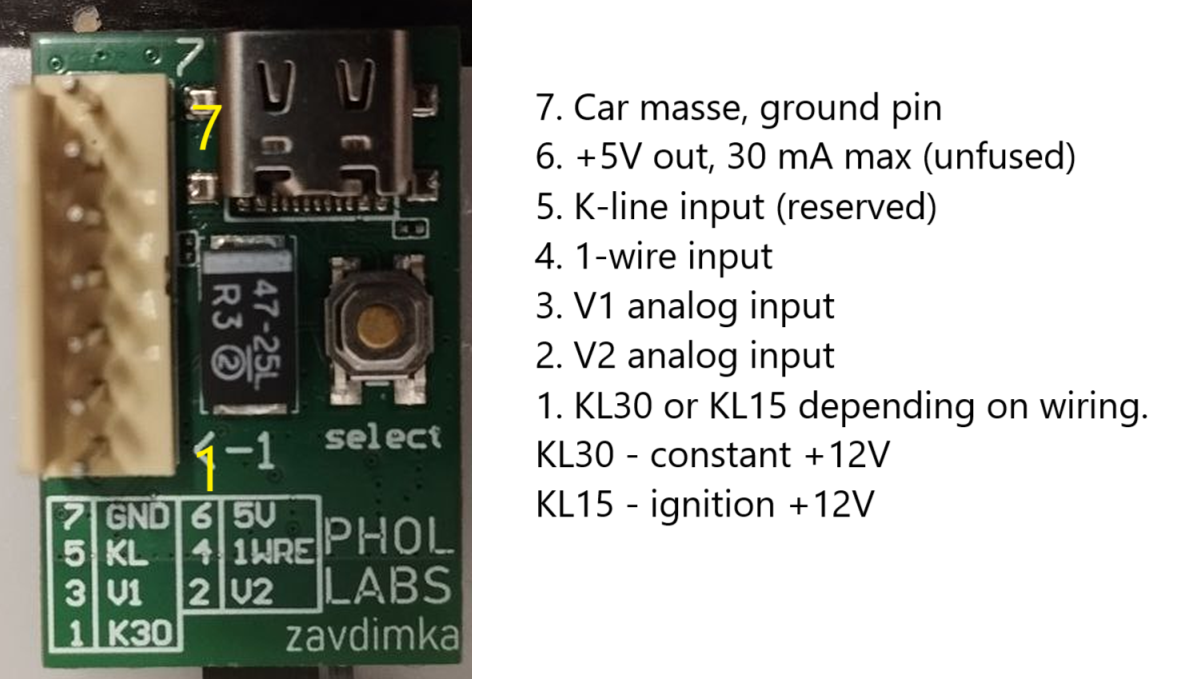
\includegraphics[width=.85\textwidth,height=.60\textheight,keepaspectratio]{figures/ivevo/image20.png}
\caption{Stecker und Anschlusspläne}
\end{figure}
\clearpage
\section{Voltmeter}

\begin{figure}[H]
\centering
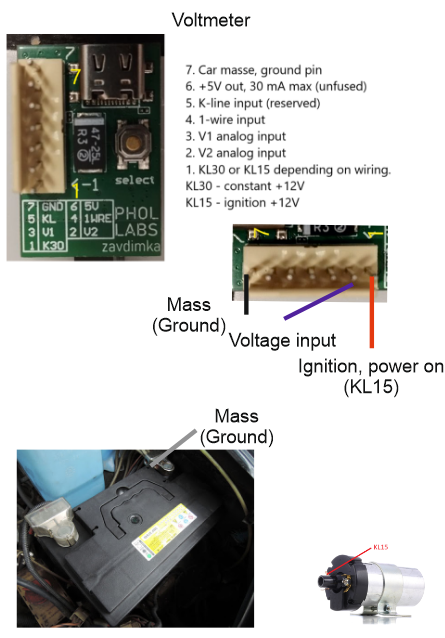
\includegraphics[width=.85\textwidth,height=.60\textheight,keepaspectratio]{figures/ivevo/image5.png}
\caption{Voltmeter}
\end{figure}
\clearpage
\section{Ganganzeige}

\begin{figure}[H]
\centering
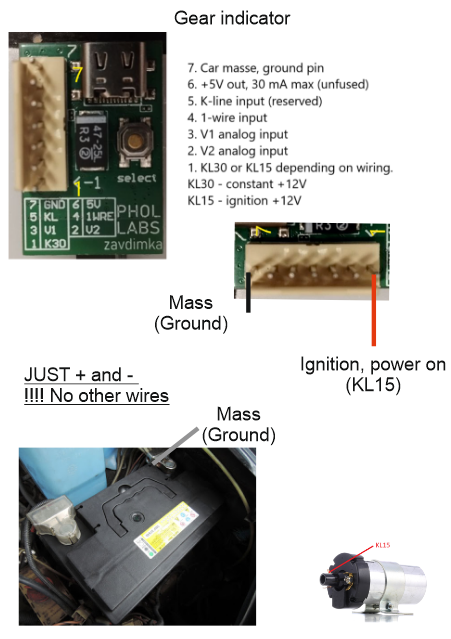
\includegraphics[width=.85\textwidth,height=.60\textheight,keepaspectratio]{figures/ivevo/image6.png}
\caption{Ganganzeige}
\end{figure}
\clearpage
\section{Öldruck}

\begin{figure}[H]
\centering
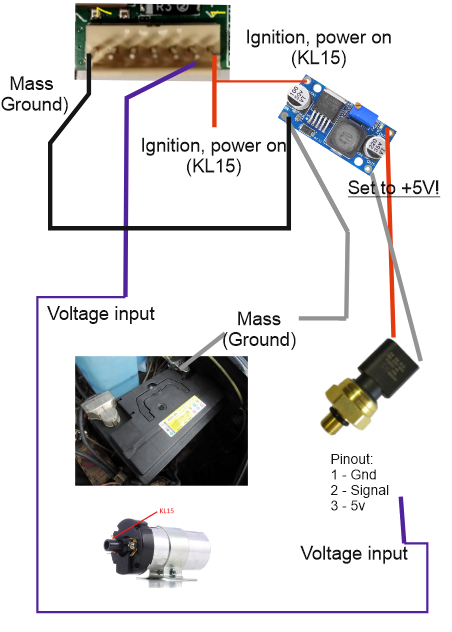
\includegraphics[width=.85\textwidth,height=.60\textheight,keepaspectratio]{figures/ivevo/image1.png}
\caption{Öldruck}
\end{figure}
\clearpage
\section{NTC-Thermometer}

\begin{figure}[H]
\centering
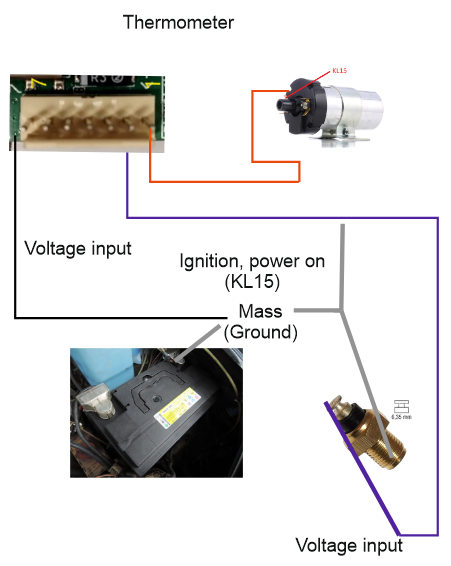
\includegraphics[width=.85\textwidth,height=.60\textheight,keepaspectratio]{figures/ivevo/image13.png}
\caption{NTC-Thermometer}
\end{figure}
\clearpage
\section{Digitalthermometer}

\begin{figure}[H]
\centering
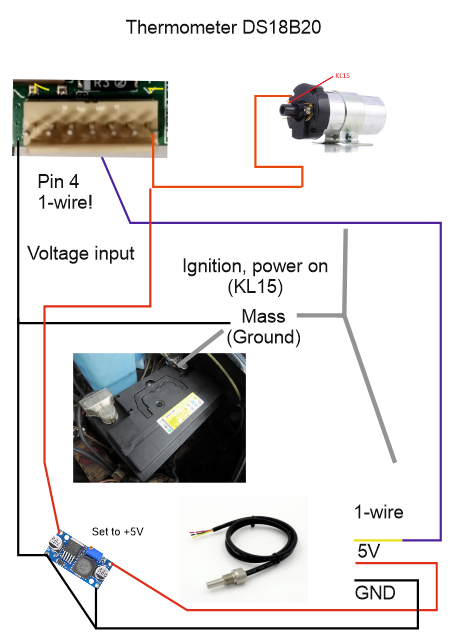
\includegraphics[width=.85\textwidth,height=.60\textheight,keepaspectratio]{figures/ivevo/image8.png}
\caption{Digitalthermometer}
\end{figure}
\clearpage
\section{Breitband-Lambda}

\begin{figure}[H]
\centering
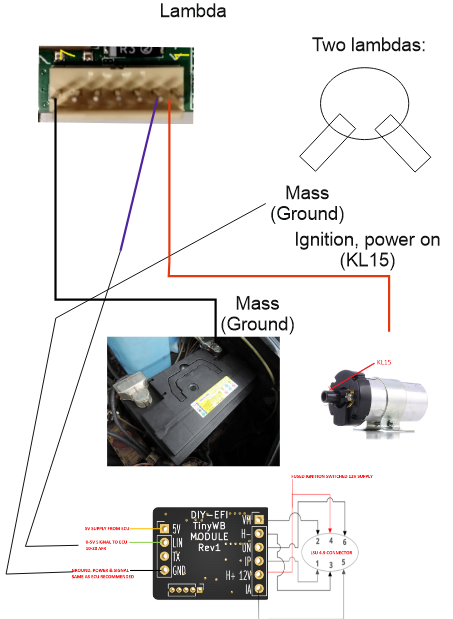
\includegraphics[width=.85\textwidth,height=.60\textheight,keepaspectratio]{figures/ivevo/image3.png}
\caption{Breitband-Lambda}
\end{figure}
\clearpage
\section{Ladedruck}

\begin{figure}[H]
\centering
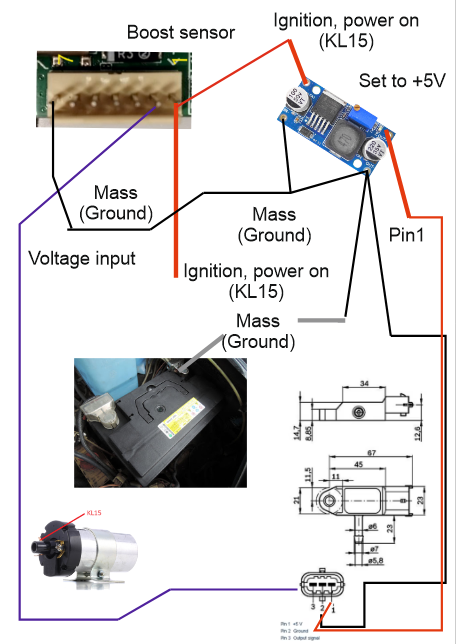
\includegraphics[width=.85\textwidth,height=.60\textheight,keepaspectratio]{figures/ivevo/image17.png}
\caption{Ladedruck}
\end{figure}
